\section{功能需求}
    \subsection{CPU}
        CPU整体工作流程图
        \begin{figure}[!hbp]
            \centering
            \caption{CPU各阶段转换图}
            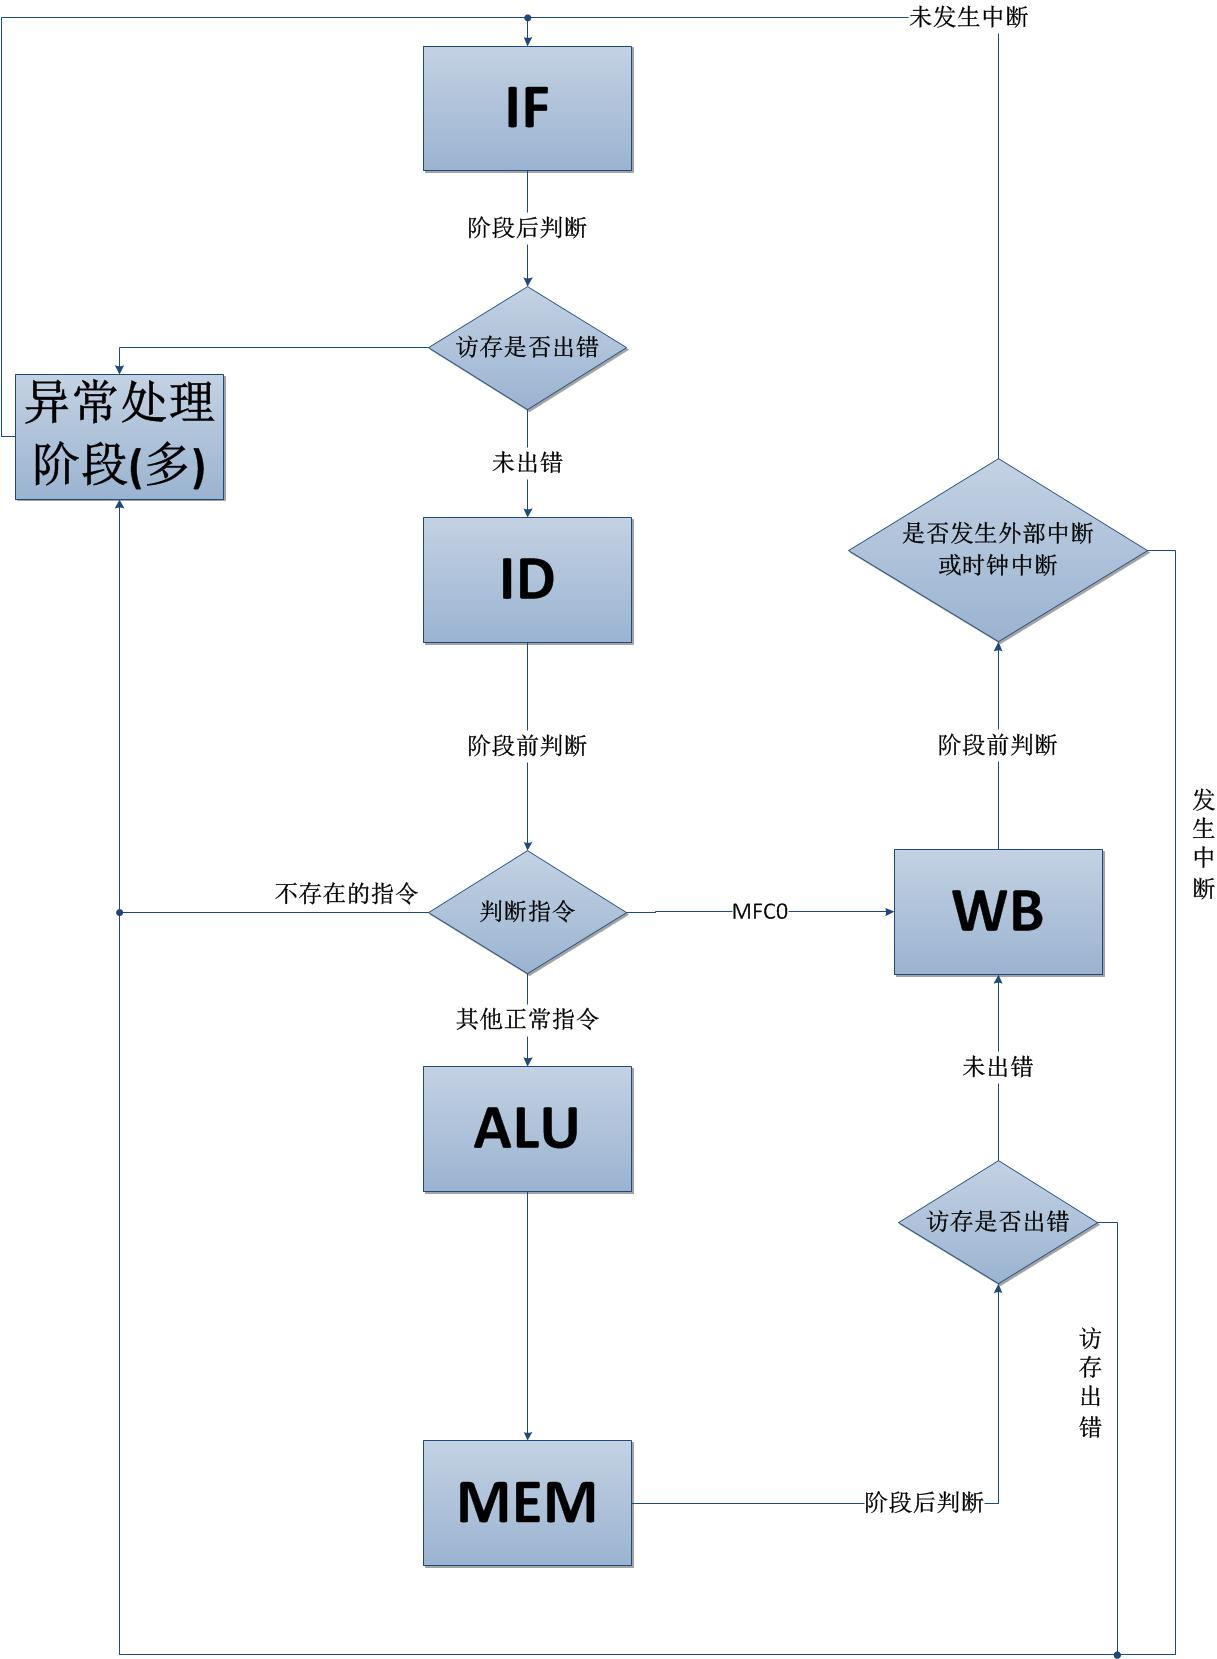
\includegraphics[width=0.75\textwidth]{chart/Stages.jpg}
        \end{figure}
                
        \subsubsection{ALU}
            功能需求:
            \begin{enumerate}
            \item
            完成数据和地址的算术、逻辑和移位运算,%
            输入两个数据根据ALUOp得出输出结果。
            \item
            根据指令系统的需求,完成指令系统中全部的算术指令(包括乘法相关指令)。
            \end{enumerate}

            实现方式:
            \begin{enumerate}
            \item
            ALU有两个输入数据,通过ALUOp生成不同结果。%
            ALUOp目前整理出17种运算,详细定义见数据通路表。
            \item
            只输出最终运算结果。不需要标志位。
            \end{enumerate}

        \subsubsection{乘法器}
            功能需求:
            \begin{enumerate}
            \item
            完成乘法功能,结果保存在LO和HI寄存器中,可以通过MT和MF类指令访问和修改计算结果。
            \end{enumerate}

            实现方式:
            \begin{enumerate}
            \item
            乘法直接使用VHDL语言中提供的乘运算符实现。
            \item
            直接与主ALU相结合,在ALUOp中加入乘法的操作码,实现乘法的计算。
            \item
            乘法指令需要的计算时间较长,但是只要时钟频率低于$50MHz$,%
            都可以在一个时钟周期内完成运算。%
            因此,在预定的时钟频率下,%
            乘法运算对时钟周期数的需求与其他运算相同,%
            暂不考虑为乘法指令设计多个时钟周期的问题。
            \item
            MFLO,MFHI,MTLO,MTHI,MULT指令查看与修改。
            在ALUOp中也加入支持MTHI、MTLO的操作码,实现对LO和HI的修改。
            同时LO和HI始终处于可读的状态,连接至写回阶段,MFLO与MFHI通过对写回阶段RegValue的控制来实现。
            \end{enumerate}

        \subsubsection{CP0}
            功能需求:

            辅助操作系统对硬件进行管理。
            \begin{enumerate}
            \item
                内存管理:辅助操作系统,完成虚拟地址和物理地址的转换、不同进程之间的内存切换、用户态与内核态内存的分离
            \item
                异常处理:检测指令执行过程中可能出现的异常、对异常进行分类、记录异常出现的指令地址或错误的内存地址
            \item
                外部中断:负责检测外部中断,辅助实现CPU与外设之间的交互

            \end{enumerate}

            实现方式:
            \begin{enumerate}
                \item
                    CP0记录CPU当前状态,通过MFC0、MTC0指令等进行读写操作,与通用寄存器建立联系
                \item
                    在异常状态发生时保存异常的返回地址,异常类型等信息
                \item
                    在内存映射中对TLB表项进行支持,为TLB充填等功能提供硬件支持
                \item
                    CP0寄存器的写方式有两种:
                    \begin{enumerate}
                        \item
                            正常执行状态下,通过MTC0指令,将CP0寄存器编号,CP0写入值,
                            CP0控制信号传递给CP0寄存器,进行写入操作。
                        \item
                            异常状态下,通过异常处理模块到CP0的连接,直接将异常原因、异常指令地址、
                            访存错误地址等信息,写入cause、EPC、BadVAddr寄存器中
                    \end{enumerate}
                \item
                    CP0寄存器的读方式有两种:
                    \begin{enumerate}
                        \item
                            正常执行状态下,通过MFC0指令,将CP0寄存器编号传递给CP0寄存器,
                            之后读取的值通过写回阶段写到通用寄存器中
                        \item
                            针对TLBWI等指令对CP0寄存器的读需求(需要同时读取5个CP0寄存器),
                            将CP0寄存器与TLB相关的直接连接到MMU单元,通过TLBWI的使能信号控制写入TLB
                    \end{enumerate}
            \end{enumerate}

            CP0具体实现方式参照下面两个小节。

            此次实验中需要实现的CP0寄存器见表\ref{table_cp0_reg}

            \begin{table}
            \centering
            \caption{需要实现的CP0寄存器}\label{table_cp0_reg}
            \begin{tabularx}{\textwidth}{|l|l|X|}
            \hline
            寄存器编号 & 名称 & 功能 \\
            \hline
            0 & Index & 用于TLBWI指令访问TLB入口的索引序号 \\
            \hline
            2 & EntryLo0 & 作为TLBWI及其他TLB指令接口,管理偶数页入口 \\
            \hline
            3 & EntryLo1 & 作为TLBWI及其他TLB指令接口,管理奇数页入口 \\
            \hline
            10 & EntryHi & TLB异常时,系统将虚拟地址部分写入EntryHi寄存器中用于TLB匹配 \\
            \hline
            8 & BadVAddr & 捕捉最近一次地址错误或TLB异常(重填、失效、修改)时的虚拟地址 \\
            \hline
            9 & Count & 每隔一个时钟周期增加1,用作计时器,并可使能控制 \\
            \hline
            11 & Compare & 当Count值与Compare相等时,SI\_TimerInt 引脚是变高电平直到有数值写入Compare,用于定时中断 \\
            \hline
            12 & Status & 表示协理器的操作模式、中断使能及诊断状态 \\
            \hline
            13 & Cause & 记录最近依次异常的原因,控制软件中断请求以及中断协理派分的向量 \\
            \hline
            14 & EPC & 存储异常处理之后程序恢复执行的地址 \\
            \hline
            15 & EBase & 识别多协理器系统中不同的协理器异常向量的基地址 \\
            \hline
            \end{tabularx}
            \end{table}

        \subsubsection{MMU与TLB}
            功能需求:
            \begin{enumerate}
            \item
                实现虚拟地址(线性地址)到物理地址的转换。% 
                只对部分地址% 
                ([0x20000000$\sim$0x80000000]和[0xC0000000$\sim$0xFFFFFFFF])% 
                进行地址映射,其余部分直接映射。
            \item
                实现内核态与用户态内存的区分。
            \item
                实现相对应的异常处理:TLBS、TLBL、TLB Modified。
            \end{enumerate}

            实现方式:
            \begin{enumerate}
            \item
                \begin{figure}[!hbp]
                    \centering
                    \caption{TLB电路结构}
                    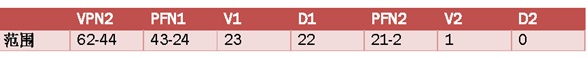
\includegraphics[width=0.9\textwidth]{chart/TLB.jpg}
                \end{figure}

                \begin{figure}[!hbp]
                    \centering
                    \caption{内存访问流程图}
                    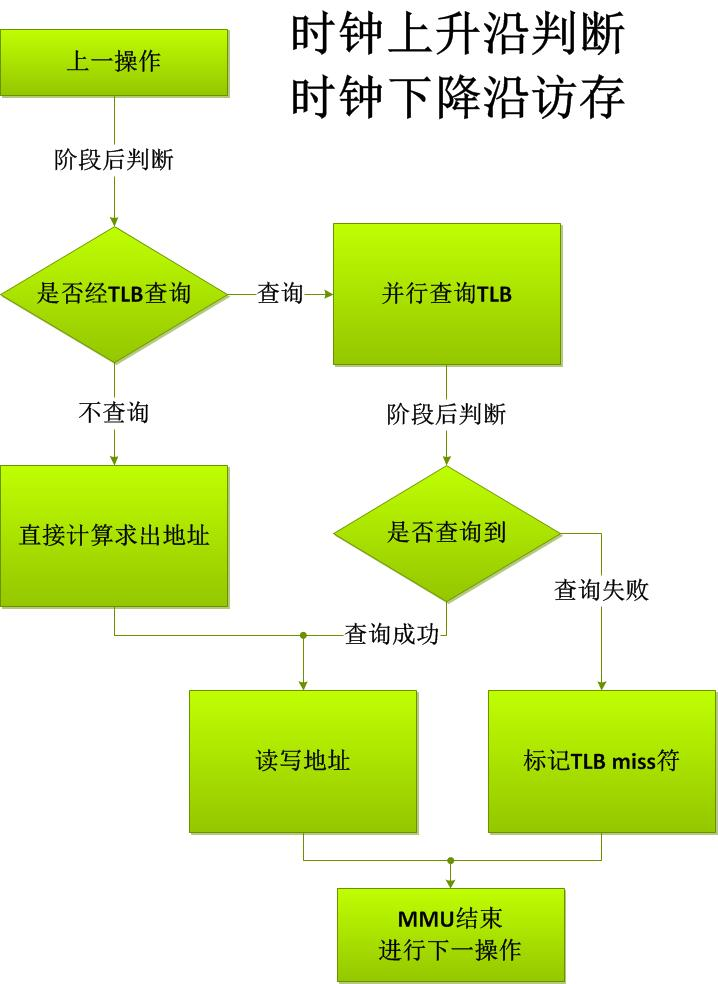
\includegraphics[width=0.4\textwidth]{chart/Memory.jpg}
                \end{figure}
                
                \begin{enumerate}
                \item
                    TLB共16项,每项可以将连续两个虚页映射到两个不同的物理页,相当于可以处理32个页
                \item
                    虚拟地址高19位作为虚页号VPN进行选择TLB表项,第20位通过奇偶判断,选择两个物理页之一
                \item
                    出于简化的考虑,不维护进程号ASID和全局标记G,默认所有G均为1,只维护每个物理地址的D和V标记
                \end{enumerate}

            \item
                硬件支持:
                \begin{enumerate}
                \item
                    虚拟地址高19位在TLB表项中并行查询EntryHi部分。
                \item
                    如果查找到,根据第20位选择EntryLo,直接与低12位结合得到真实的物理地址。
                \item
                    如果未查找到,触发TLBMiss异常:%
                    设置Cause寄存器中的ExcCode为TLB异常,%
                    EPC寄存器为当前指令的地址,%
                    BadvAddr寄存器为错误的地址,%
                    之后触发一个异常,PC跳转到EBase的异常处理基地址,%
                    之后由操作系统接管。
                \item
                    对于地址不对齐异常,在内存映射阶段对虚拟地址offset部分最低两位进行检测%
                    如果不为00,则触发地址不对齐异常,交由操作系统处理
                \end{enumerate}
            \item
                操作系统:
                \begin{enumerate}
                \item
                    进入异常处理向量0x80000180。
                \item
                    跳转到处理函数部分(trap/trapentry.S/__alltraps)。
                \item
                    先保存异常现场,之后进入trap函数(trap/trap.c)。
                \item
                    根据是否发生嵌套异常调整trapframe,%
                    之后进入trap_dispatch函数(trap/trap.c)。
                \item
                    根据cause寄存器的值进行分类,调用tlb\_miss\_handler函数。
                \item
                    得到异常地址对应的物理页号,%
                    之后进行tlb\_write(mm/tlb.c)。
                \item
                    操作系统维护index,%
                    写EntryLo0、EntryLo1、EntryHi、 PageMask、Index五个寄存器,%
                    之后用tlbwi写到TLB的第Index项。%
                    此处需要硬件提供MTC0、MFC0、TLBWI指令的支持。
                \item
                    异常返回,重新执行取地址命令。%
                \end{enumerate}
            \end{enumerate}

        \subsubsection{异常中断处理}
            功能需求:
            \begin{enumerate}
            \item
            实现对异常和外部中断的处理。
            \item
            实现的异常有内存访问异常、地址不对齐异常、%
            系统调用、未定义的指令异常、未定义的寄存器异常。
            \item
            中断:串口中断、时钟中断。
            \end{enumerate}

            实现方式:
            \begin{figure}[!hbp]
                    \centering
                    \caption{异常中断处理流程}
                    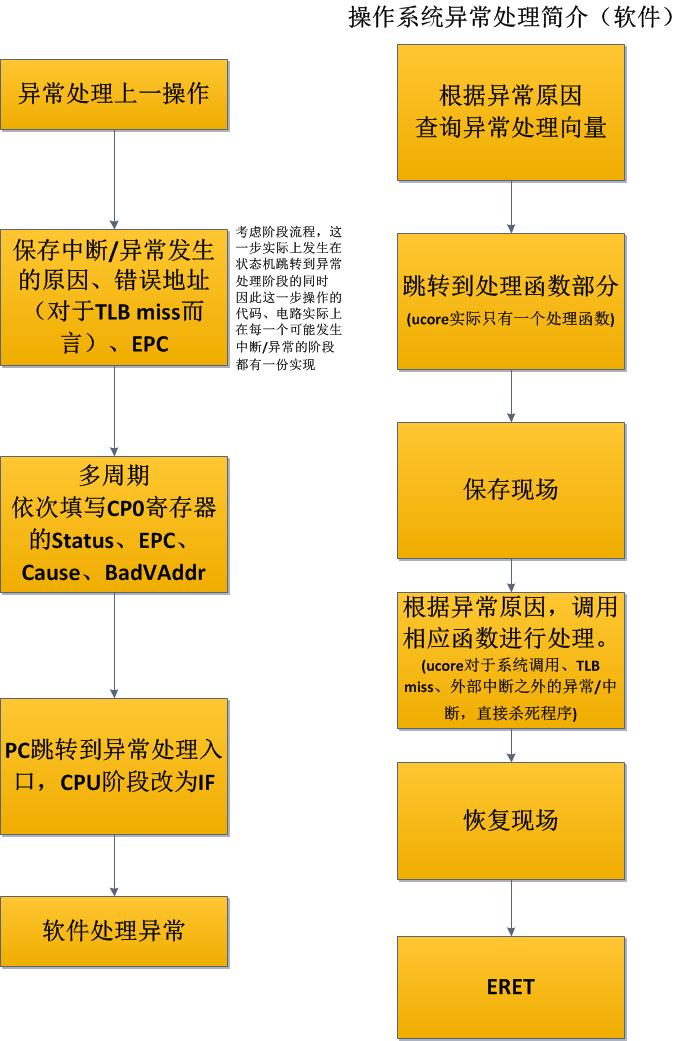
\includegraphics[width=0.5\textwidth]{chart/Exception.jpg}
            \end{figure}
            
            \begin{enumerate}
            \item
            硬件支持
                \begin{enumerate}
                \item
                异常处理,在数据通路上添加异常处理部分,%
                在多周期的任意一个周期检测到异常后,%
                在Cause设置异常代码、%
                在EPC寄存器设置异常处理的返回地址,%
                将Status寄存器的EXL为设置为1,表示进入内核态处理异常%
                之后根据EBase跳转到异常处理向量基地址,%
                之后操作系统接管。
                \item
                外部中断处理,设置外部中断检查信号,外部设备触发时,%
                异步地将检查信号置1;每个指令IF阶段检查该信号,%
                若为1则进入外部中断处理,否则正常执行指令。
                \item
                时钟中断处理。当寄存器Count和Compare寄存器中的数值相等时,%
                触发一个时钟异常,交由操作系统处理。
                \end{enumerate}
            \item
            操作系统
                \begin{enumerate}
                \item
                进入异常处理向量0x80000180。
                \item
                跳转到处理函数部分(trap/trapentry.S/__alltraps)。
                \item
                先保存异常现场,之后进入trap函数(trap/trap.c)。
                \item
                根据是否发生嵌套异常调整trapframe,%
                之后进入trap_dispatch函数(trap/trap.c)。
                \item
                根据cause寄存器的值进行分类,%
                调用cons\_getc、syscall等等函数进行处理,%
                如果是地址不对齐异常,或者未定义的异常,直接退出。%
                如果是未定义的指令异常,可能是除法指令所导致的,%
                通过ri\_handler函数尝试进行模拟除法,%
                如果仍然不能得到正确结果则退出程序。
                \item
                使用ERET指令从异常返回,将EXL位重新设置为0,表示进入用户态
                重新执行取地址命令
                \end{enumerate}
            \end{enumerate}

            \begin{table}
            \centering
            \caption{需要实现的异常}
            \begin{tabular}{|c|c|c|}
            \hline
            异常号 & 异常名 & 描述 \\
            \hline
            0 & Interrupt & 外部中断,异步发生,由硬件引起 \\
            \hline
            1 & TLB Modified & 内存修改异常, 发生在Memory阶段 \\
            \hline
            2 & TLBL & 读未在TLB中映射的内存地址触发的异常 \\
            \hline
            3 & TLBS & 写未在TLB中映射的内存地址触发的异常 \\
            \hline
            4 & ADEL & 读访问一个非对齐地址触发的异常 \\
            \hline
            5 & ADES & 写访问一个非对齐地址触发的异常 \\
            \hline
            8 & SYSCALL & 系统调用 \\
            \hline
            10 & RI & 执行未定义指令异常 \\
            \hline
            \end{tabular}
            \end{table}

        \subsubsection{其他功能部件}
            \paragraph{PC}
                \mbox{} \\ 

                功能需求:
                \begin{enumerate}
                \item
                实现PC的多种变换方式:正常执行、分支、跳转。
                \item
                实现异常处理时对PC的处理,跳转到异常处理向量部分。
                \end{enumerate}

                实现方式
                \begin{enumerate}
                \item
                在写回模块对PC进行操作,将立即数或寄存器的值与当前PC进行运算%
                实现PC的多种变化方式。%
                决定是否跳转的比较操作也在这一模块完成。
                \item
                针对异常状态、从异常返回两种情况的PC变化,从CP0寄存器中引出EPC与EBase两个地址到PC计算单元。
                通过当前的状态进行判断PC的取值。
                \item
                下一条指令的PC在本条指令的写回阶段得到确定,
                保证在下一条指令的取指令时钟上升沿开始之前,正确送到MMU进行取指令。
                \end{enumerate}

            \paragraph{寄存器堆}
                \mbox{} \\ 

                功能需求:
                \begin{enumerate}
                \item
                实现通用寄存器,以及在数据通路中的读写控制。
                \end{enumerate}

                实现方式
                \begin{enumerate}
                \item
                在CPU中实现寄存器堆并实现读写控制。
                \item
                在解码指令阶段,根据指令的rs、rt、rd位置读取通用寄存器。
                与写回模块相配合,完成寄存器堆的写入
                \end{enumerate}

            \paragraph{串口}
                \mbox{} \\

                功能需求:
                \begin{enumerate}
                \item
                实现与PC机通信,通过计算机键盘输入数据,向计算机输出数据。
                \end{enumerate}

                实现方式
                \begin{enumerate}
                \item
                使用开源的%
                \href{http://www.fpga4fun.com/SerialInterface.html}{ASync transmitter and receiver},%
                通过在每个信号周期内多次采样,并滤波得到稳定的信号。%
                CPLD仅负责TX/RX端口数据的转发,%
                对数据的编码与解码在FPGA中进行。%
                这样设计提高了数据传送的准确率,%
                并且串口数据不需要占用内存数据线,%
                无需处理冲突,简化了设计。%
                数据通信协议在开发过程中设计,有待进一步说明。

                \end{enumerate}
        \subsubsection{扩展部分}
            在开发过程中测试是必不可少的环节,%
            因此,此次实验的扩展部分计划实现一个类似gdb的工具,%
            并给出一份较为详细的测试方案。

            调试工具在电脑端提供与gdb类似的终端,%
            支持gdb中的print、break等基本命令。%
            在硬件上,通过串口进行指令的输入与数据的输出,%
            尽可能减少对原有CPU设计的修改。
            
            在每个模块正常工作之后,将各个模块进行组合,形成整体的CPU设计。%
            通过操作系统的lab循序渐进地对CPU进行测试,%
            此时可以使用开发的类gdb工具,%
            设置断点、输出信号进行调试。
            
        \subsubsection{指令集与数据通路}
            指令集为标准MIPS系统子集

            实现多周期CPU,针对指令集设计数据通路。
            仿照《软件硬件接口》书中的多周期CPU进行设计,
            在书中7条指令的原型上进行扩展,以支持标准MIPS系统的子集。
            
            指令执行过程主要分为取指、解码、执行、访存、写回五个周期,
            某些指令可能需要其他特殊的周期支持,采用多周期实现比较灵活。

            数据通路包括状态机与控制线设计,每条指令有不同的状态机变化,
            而且对指令进行解码,能够得到相应的控制线。%
            在多周期的不同周期利用控制线对数据通路进行控制,使指令正常执行。
            
            数据通路图在设计文档中有详细体现。

            
    \subsection{BIOS}
        准备阶段:
        \begin{enumerate}
            \item
                操作系统和文件系统烧写到Flash中%
            \item
                编译出的二进制文件写到ROM中
            \item
                CPU代码烧写到FPGA中。
        \end{enumerate}

        启动阶段:
        \begin{enumerate}
            \item
                从ROM中的bootasm.S启动
            \item
                将Flash中的全部操作系统拷贝到RAM中,然后控制权交给操作系统。
        \end{enumerate}

        操作系统启动阶段:
        \begin{enumerate}
            \item
                bootasm.S工作结束后,进入操作系统entry.S文件中进行寄存器初始化。
            \item
                entry.S:通用寄存器清零,CP0寄存器设置为默认值,异常处理基地址进行初始化,之后跳转到init.c中的kern\_init。
            \item
                kern\_init:完成TLB初始化(全部TLB表项清零),物理内存与虚拟内存的转换页表的初始化(创建初始页表)
            \item
                最后完成操作系统的进程和文件管理系统,至此ucore系统开始正常工作,
        \end{enumerate}
        

